\documentclass[conference]{IEEEtran}
\IEEEoverridecommandlockouts
% The preceding line is only needed to identify funding in the first footnote. If that is unneeded, please comment it out.
\usepackage{cite}
\usepackage{amsmath,amssymb,amsfonts}
\usepackage{algorithmic}
\usepackage{graphicx}
\usepackage{textcomp}
\usepackage{xcolor}

\usepackage{threeparttable}
\usepackage{tabularx,booktabs}
\usepackage{siunitx}
  \sisetup{
    table-format=1.3,
    round-mode = places,
    round-precision = 3,
  }
\usepackage{kantlipsum}

\usepackage{capt-of}
\usepackage{cuted}   

\def\BibTeX{{\rm B\kern-.05em{\sc i\kern-.025em b}\kern-.08em
    T\kern-.1667em\lower.7ex\hbox{E}\kern-.125emX}}
\begin{document}

\title{Vergleich verlustfreier Datenkompressionsverfahren auf Bilddaten}

\author{
    \IEEEauthorblockN{Nick Schreiber}
    \IEEEauthorblockA{Technische Hochschule Rosenheim\\
        Master Informatik, Seminar theoretische Informatik\\
        Email: nick.schreiber@stud.th-rosenheim.de}
}

\maketitle

\begin{abstract}
    This document is a model and instructions for \LaTeX.
    This and the IEEEtran.cls file define the components of your paper [title, text, heads, etc.]. *CRITICAL: Do Not Use Symbols, Special Characters, Footnotes,
    or Math in Paper Title or Abstract.
\end{abstract}


% \begin{IEEEkeywords}
% component, formatting, style, styling, insert
% \end{IEEEkeywords}

\section{Einleitung}

Datenkompression beschreibt ein Verfahren, das zum Ziel hat, eine Nachricht
ohne relevanten Informationsverlust zu verkleinern.
Als Nachricht ist jede Art von digitalen Daten gemeint, z.B. Text, Bild, Audio, etc..
Daten können komprimiert werden, indem Redundanz entfernt oder eine Kodierung angewendet wird.
Daher wird Datenkompression oft als Kodierung bezeichnet.
Kodierung ist ein allgemeiner Begriff, der jede spezielle Darstellung von Daten nach
einem bestimmten Schema umfasst. \cite{Ingles}

Es gibt zwei Arten der Datenkompression: die verlustbehaftete und die verlustfreie Kompression.
Bei der verlustbehafteten Datenkompression kann eine bestimmte Menge an Information durch die
Kompression verloren gehen, was in Kauf genommen wird, da dadurch die Datenmenge erheblich
reduziert werden kann oder weil die verlorene Informationen für die Anwendung kaum relevant sind.
Das wird auch als Irrelevanzreduktion bezeichnet \cite[S. 5]{Maluck}.
Ein Beispiel für Irrelevanzreduktion kann bei Audiosignalen beobachtet werden.
Der menschliche Hörfrequenzbereich liegt zwischen 20 Hz und 20 kHz \cite{Burke}.
Daher ist es nicht sinnvoll, Frequenzen, die weit außerhalb des hörbaren Bereichs liegen,
in Audiodateien zu speichern.
Bei der verlustfreien Datenkompression wird die Integrität der Daten bewahrt.
Das bedeutet, dass sämtliche Informationen in den komprimierten Daten enthalten sind
und die Originaldaten vollständig rekonstruierbar sind.
In dieser Arbeit wird nur die verlustfreie Datenkompression untersucht, da
Irrelevanzreduktion nicht direkt zum Themengebiet der Datenkompression gehört.

Die Datenkompression von Bildern wird aus verschiedenen Gründen eingesetzt.
Speichernutzung: Unkomprimierte Bilddaten können beträchtlich mehr Speicherplatz beanspruchen.
Übertragungseffizienz: Bei der Übertragung von Bildern über Netzwerke oder das Internet spielt
die Übertragungseffizienz eine entscheidende Rolle.
Wenn ein Bild über einen Kanal mit begrenzter Bandbreite gesendet wird, kann es effizienter
sein, das Bild zu komprimieren, es zu übertragen und dann beim Empfänger zu dekomprimieren.
Dadurch wird die Übertragungszeit verkürzt und das Bild kann schneller bereitgestellt werden.
Dies führt zu einer höheren Übertragungsrate und einer reduzierten Bandbreitennutzung.



\section{Zielsetzung der Arbeit}

Ziel der Arbeit ist es zu untersuchen, ob und warum bestimmte verlustfreie
Datenkompressionsverfahren für Bilddaten besser geeignet sind als andere.
Dazu werden die theoretischen Aspekte der Kompressionsalgorithmen untersucht.
Außerdem wird untersucht, wie Bilddaten aufgebaut sind und welche Besonderheiten
in den Bilddaten für die Datenkompression genutzt werden können.
Die Arbeit hat einen praktischen Anteil.
Verschiedene Algorithmen zur verlustfreien Datenkompression wurden manuell
implementiert und an unterschiedlichen Bilddaten getestet.
So konnten konkrete Ergebnisse über die Leistungsfähigkeit der Algorithmen gewonnen werden.
Die verglichenen Algorithmen sind Run Length Encoding (RLE), Huffman Encoding,
Lempel-Ziv 1977 (LZ77), PNG Algorithmus und verschiedene Kombinationen der Algorithmen.
Die Ergebnisse werden interpretiert und mit den theoretischen Erwartungswerten verglichen.

% Todo ab hier nochmal verbessern!
\section{Grundlagen zur Datenkompression}

In der Informatik gehört die Datenkompression zum Teilgebiet der Informationstheorie.
Um zu verstehen, wie verlustfreie Datenkompression funktioniert, muss man einige theoretische
Grundlagen kennen.

\subsection{Information}

Claude Shannon, der Erfinder der Informationstheorie, definiert den Begriff Information
als Maß für den Informationsgehlt.
Information ist ein Maß der Unsicherheit, das durch das Eintreten eines bestimmten
Ereignisses oder das Empfangen einer Nachricht verringert wird. \cite{shannon}
Information ist die Mindestanzahl von Bits, die zur Codierung einer Nachricht verwendet
werden müssen. \cite{shannon2}
Die grundlegende Idee zu Information besteht darin, dass Informationen umso wertvoller sind,
je unerwarteter oder unwahrscheinlicher sie sind.

\subsection{Entropie}

Die Quantifizierung des Informationsgehalts erfolgt durch die Entropie ($H$).
Formal drückt die Entropie die durchschnittliche Menge an Bits aus,
die benötigt werden, um eine Information zu kodieren. \cite{shannon}
Die Entropie berücksichtigt die Wahrscheinlichkeiten verschiedener möglicher
Ereignisse und erreicht ein Maximum, wenn alle Ereignisse gleich wahrscheinlich sind,
was auf maximale Unsicherheit hinweist.

\begin{equation}
    \label{eq:entropie}
    H(X) = -\sum_{i=1}^{n} P(x_i) \cdot \log_{2}(P(x_i))
\end{equation}

Formel \ref{eq:entropie} definiert die Entropie mathematisch.
Hierbei steht $H(X)$ für die Entropie der Menge $X$.
$P(x_i)$ steht für die Wahrscheinlichkeit des
Auftretens des Ereignisses $x_i$.
Die Summe wird über alle möglichen Ereignisse
$x_i$ in $X$ gebildet.

Diese Formel beschreibt die durchschnittliche Menge an Bits, die benötigt werden,
um eine Nachricht aus X zu kodieren.
Wenn die Entropie hoch ist, ist die Unsicherheit groß, und es werden mehr Bits
benötigt, um die Informationen zu repräsentieren.
Wenn die Entropie niedrig ist, gibt es weniger Unsicherheit, und somit werden
weniger Bits benötigt.

Man kann nun eine direkte Verbindung zwischen Entropie und Kompression herzustellen.
Niedrige Entropie bedeutet, dass eine Datenmenge strukturiert ist, bzw. Muster aufweist.
Das heißt, dass in den Daten wenig unsicherheit ist und die Daten Redundanz enthalten.
Das bedeutet, niedrige Entropie sagt, dass die Daten komprimiert werden können.


\subsection{Redundanz und Mutual Information}

Redundanz beschreibt Informationen die in Daten mehrfach vorhanden sind. \cite{friedrichs}
Einfach gesagt kann man Redundanz als überflüssige Information betrachten.
Eine hohe Redundanz sagt aus, dass sich wiederholende oder vorhersehbare Muster innerhalb
der Daten befinden.

Um eine Formel für die Redundanz aufzustellen benötigt man die mittlere Codewortlänge.
Die mittlere Codewortlänge gibt den durchschnittlichen Bedarf an Bits pro Symbol in einer
Nachricht an.
Sei $X$ ein Alphabet und $x \in X$.
$C(x)$ bezeichnet das zu $x$ gehörende Codewort.
$l(x)$ bezeichnet die Länge von $C(x)$.
Die mittlere Codewortlänge L(C) einer Nachricht C(x) mit der Wahrscheinlichkeitsverteilung
p(x) ist in Formel \ref{eq:codewortlänge} definiert.

\begin{equation}
    \label{eq:codewortlänge}
    L(C) = \sum_{i}^{|X|} p(x_i) \cdot l(x_i)
\end{equation}

Mit der mittleren Codewortlänge lässt sich nun die Redundanz des Codes, bzw. der
Nachricht berechnen.
Die Formel \ref{eq:redundanz} definiert die Redundanz einer Nachricht.

\begin{equation}
    \label{eq:redundanz}
    R_{\text{Code}} = L(C) - H(X)
\end{equation}

Die Redundanz wird berechnet, indem von der tatsächlichen durchschnittlichen
Anzahl an Bits pro Symbol die theoretisch minimale Anzahl an Bits pro Symbol
abgezogen werden.
Die theoretisch minimale Anzahl an Bits pro Symbol entspricht der enthaltenen
Information und ist gleich der Entropie der Nachricht.
Daraus ergibt sich, dass die Redundanz $\geq$ 0 sein muss.

Mutual Information ist ein quantitatives Maß für die gegenseitige Abhängigkeit von zwei
Variablen. \cite{shannon}
Es misst, wie sehr die Kenntnis einer Variablen die Unsicherheit über die andere
Variable reduziert.
Dieses Konzept ist entscheidend, um die Struktur von Daten zu verstehen und
voneinander abhängige Informationen zu erkennen.

Wenn die Mutual Information zwischen zwei Variablen hoch ist, bedeutet dies,
dass das Wissen über eine Variable
bedeutende Informationen über die andere Variable liefert.
Hohe Mutual Information sagt dementsprechend aus, dass zwei Variablen stark voneinander
Abhängig sind.
Das Wissen über den Wert einer Variable trägt bereits wesentlich zur Vorhersage
oder zum Verständnis der anderen Variable bei.

Geringe Mutual Informaion sagt aus, dass die beiden Variablen weniger gemeinsame
Information teilen.
Das Wissen über den Wert einer Variable trägt nicht so stark zur
Vorhersage oder zum Verständnis der anderen Variable bei.
Das bedeutet eine schwächere Statistische Abhängig der Variablen.

Durch das erkennen von Mutual Information kann gezeigt werden, dass Muster und/ oder
Wiederholungen und dementsprechend Redundanz in den Daten enthalten ist.
Redundanz spielt im Bezug auf Kompression eine wichtige Rolle.
Kompression funktioniert durch das identifizieren und eliminieren redundanter Elemente,
um den Informationsgehalt zu maximieren und die Effizienz von Datenrepräsentationen
zu steigern.


\section{Informationstheorie}

Eine wichtige Punkt in der Informationstheorie ist die Unterscheidung
zwischen Daten und Information.
Daten und Information werden im normalen Sprachgebrauch häufig als Synonym verwendet,
was eigentlich nicht korrekt ist.

Daten sind rohe Fakten oder Symbole, die an sich keine spezifische Bedeutung haben.
Informationen entstehen durch die Interpretation, Organisation und Strukturierung
von Daten, wodurch ein sinnvoller Kontext geschaffen wird. \cite{pieper}
Daten werden zu Informationen, wenn sie für einen bestimmten Zweck verwendet werden können.

Im Kontext der Datenkompression ist es wichtig zu verstehen, dass nicht alle Daten
gleichermaßen informativ sind.
Ein effektiver Kompressionsalgorithmen entfernt redundante
und nicht informative Teile der Daten.
Jedoch bleibt die gesamte Information enthalten.
Die Daten sind somit invormativer und komprimierter als zuvor.

\subsection{Quellencodierungstheorem/ Source Coding Theorem}

Das Quellencodierungstheorem beschäftigt sich mit der Effizienz der Datenkompression
und sagt aus, dass es eine Grenze für die minimale mittlere Codierungslänge gibt,
die für die Darstellung von Information aus einer bestimmten Quelle erforderlich
ist. \cite{sharma}
Das Quellencodierungstheorem besagt, dass die mittlere Codierungslänge $L$ pro Symbol
für eine gegebene Quelle nicht kleiner sein kann als die Entropie $H$ der Quelle.
Mathematisch in Formel \ref{eq:sct} ausgedrückt.

\begin{equation}
    \label{eq:sct}
    L \ge H
\end{equation}

Die Entropie stellt dabei die untere Schranke für die mittlere Codierungslänge dar.
Das zeigt, dass Datenkompression nicht bis ins unendliche möglich ist ohne
Information zu verlieren.
Die Maximale Kompression ist genau dann erreicht, wenn $L = H$ entspricht.
Es würde also bei solchen Daten keinen sinn machen zu versuchen die Daten
zu komprimieren, da das ohne Informationsverlust nicht möglich ist.

Vlt. Todo: Schubfachprinzip, Bedeutung von Entropie in diesem Kontext.

\subsection{Kolmogorov Komplexität}

Die Kolmogorov Komplexität ist ein Maß für die Strukturiertheit einer Zeichenkette.
Sie entspricht der Länge des kürzesten Programms, das die Zeichenkette erzeugen
kann. \cite{li}
Die Kolmogorov Komplexität ist dementsprechend ein Maß für die algorithmische Komplexität
von Informationen.

Die Kolmogorov Komplexität eines Objekts, z. B. eines Textes, ist die Länge
des kürzesten Programms, das das Objekt als Ausgabe erzeugt.
Hier ein Beispiel für so ein Programm.
Betrachten wir die folgende Zeichenkette: "AAAAAAAAABBBBBCCCCCC".
Die Zeichenkette besteht aus 20 Zeichen (9 x A, 5 x B, 6 x C).
Mit einem einfachen Programm lässt sich die Zeichenkette deutlich kürzer
beschreiben: "9A5B6C".
Das Programm gibt die Länge der identischen aufeinanderfolgenden Zeichen an,
gefolgt von dem Zeichen.
So lässt sich die ursprüngliche Zeichenkette der Länge 20 in nur 6 Zeichen darstellen.
Wir haben ein Programm gefunden, das die Länge der Beschreibung der Zeichenkette
erheblich reduziert.
Die Kolmogorov Komplexität dieser Zeichenkette ist deutlich geringer als
die ursprüngliche Länge der Zeichenkette.
Das zeigt, dass in der Zeichenkette Strukturen vorhanden sind.

Es ist wichtig zu beachten, dass die tatsächliche Kolmogorov Komplexität für
allgemeine Zeichenketten wegen des Halteproblemes nicht praktisch
berechenbar ist. \cite{OPPaper}
Allerdings können Abschätzungen gemacht werden.
Wenn ein Algorithmus gefunden wird, der eine Zeichenkette in einem kürzeren
Programm darstellt entspricht die Kolmogorov Komplexität der Zeichenkette
maximal der Länge des Programms.
Es ermöglicht den Informationsgehalt von Daten in
Bezug auf die kürzeste mögliche algorithmische Beschreibung zu verstehen.

% Eine enge Verbindung besteht zur Vorstellung
% der optimalen, universellen Datenkompression – je einfacher die Beschreibung, desto
% effizienter kann die Datenmenge komprimiert werden.
% Dieses Konzept hat weitreichende praktische Anwendungen, von der Identifikation von
% wiederholten Mustern bis hin zur Bewertung von Algorithmeneffizienz.
% Allerdings stehen der Anwendung auch Herausforderungen gegenüber, wie der Unberechenbarkeit
% des absoluten Komplexitätsmaßes und der Schwierigkeit, universelle Algorithmen zu finden,
% die für alle Daten gleichermaßen effizient sind. Das Verständnis der Kolmogorov-Komplexität
% trägt maßgeblich zur Entwicklung fortgeschrittener Datenkompressionsverfahren bei und bietet
% Einblicke in die Grenzen der Komprimierbarkeit von Informationen.

% Anforderungen an Daten, damit diese komprimierbar sind
\subsection{Datenanforderungen, Komprimierbarkeit}

Daten können in verschiedene Gruppen eingeteilt werden.
Auf der einen Seite stehen strukturierte Daten und auf der anderen Seite
unstrukturierte Daten.

Strukturierte Daten sind Daten in denen wiederkehrende oder vorhersagbare Muster
enthalten sind.
Die Entropie der Daten ist niedrig.
Ein Beispiel für strukturierte Daten sind Tabellen.

Unstrukturierte Daten sind Daten, in denen keine wiederkehrende oder vorhersagbare
Muster enthalten sind.
Die Entropie der Daten ist hoch.
Ein Beispiel für unstrukturierte Daten sind zufällig erzeugte Daten.

Strukturierte Daten enthalten meist eine höhere Redundanz als unstrukturierte
Daten.
Das ist dem Fakt geschuldet, dass die maximal mögliche Kompression, der Information in den
Daten, der Entropie, entspricht.
Daten können theoretisch maximal auf das Niveau der Entropie der Daten komprimiert werden.
Strukturierte Daten mit geringer Entropie haben ein tieferes Limit als unstrukturierte Daten.
Deshalb können strukturierte Daten meist mehr komprimiert werden als unstrukturierte.

\subsubsection{Vorverarbeitung}

Eine Möglichkeit aus etwas unstrukturierten Daten strukturiertere zu machen ist über
eine Vorverarbeitung der Daten.
So eine Vorverarbeitung ist meist eine Normalisierung oder eine Datenfilterung.
Wichtig ist, dass der Vorverarbeitungsschritt umkehrbar ist.
Eine Art wie Daten für die Kompression Vorverarbeitet werden, wird im Lauf der
Arbeit anhand des PNG Algorithmus gezeigt.
PNG verwendet eine Datenfilterung.

\subsubsection{Limitationen}

Ein Beispiel für maximal unstrukturierte Daten die scheinbar nicht komprimierbar
sind, sind normalverteilte Zufallszahlen.
"The Random Compression Challenge" von Mark Nelson \cite{nelson} betrachtet genau dieses
Problem.
Das Ziel der Challenge ist es eine Datei, die etwa ein halbes Megabyte groß ist
zu komprimieren.
Die Datei besteht aus einer Millionen Zufallszahlen, die gleichverteilt sind und
aus dem Buch "A Million Random Digits with 100,000 Normal Deviates" \cite{amilli}
kommen.

Es gibt zwei Arten wie die Challenge gewonnen werden kann.
Die eine Möglichkeit ist es, die Kolmogorov Komplexität zu verwenden und ein
Programm zu schreiben, dass die ursprüngliche Datei erzeugt.
Die größe des Programms muss kleiner sein, als die zu komprimierende Datei.
Es geht dabei darum zu zeigen, dass die Kolmogorov Komplexität kleiner ist
als die Größe der Datei selbst.

Die andere Möglichkeit ist es, ein System zu entwickeln, dass Dateien mit normalverteilten
Zufallszahlen komprimieren und vollständig wieder aus der komprimierten Datei
dekomprimieren kann.
Die größe des Systems spielt dabei keine Rolle, weil das System mehr als nur eine
Datei erfolgreich komprimieren und dekomprimieren muss.
Es ist bewiesen, dass dieser Ansatz unmöglich ist \cite{nelson}.
Der Grund dafür ist, dass die Entropie der größe der Datei selbst entspricht und
ohne Informationsverlust nicht verkleinert werden kann.

Bis heute hat noch niemand die Challenge gewonnen.
Das ist nicht verwunderlich, da
die zweite Möglichkeit zu gewinnen bewiesenermaßen unmöglich ist.
Hingegen ist die erste Möglichkeit mit dem Kolmogorov Komplexität nur
vermutlich unmöglich.
Das bedeutet es könnte eine Lösung geben, ist aber nach jetzigem Stand unwahrscheinlich.

Die Challenge ist ein perfektes Beispiel dafür, wieso es Sinn macht die Daten zu
kennen die man komprimieren will.
Sie zeigt die Limitationen der Datenkompression auf.


\section{Aufbau und Struktur von Bilddaten}

Dieser Abschnitt beschäftigt sich mit der dem Aufbau und der Struktur von Bilddaten.
Es gibt verschiedene Möglichkeiten Bilddaten zu speichern und darzustellen.
In dieser Arbeit werden die Bilder in Form einer Rastergrafik/ Bitmap gespeichert, dem
RGB Format.
Eine Rastergrafik ist eine pixelbasierte Darstellung eines Bildes.
Die Auflösung eines Bildes gibt an, wie viele Pixel in der Breite und Höhe vorhanden sind.
Ein Pixel ist die kleinste diskrete Einheit in einem digitalen Bild.

Das RGB Format ist eine Möglichkeit, Farbinformationen in digitalen Bildern zu
repräsentieren und zu speichern.
RGB steht für die Farben Rot (R), Grün (G) und Blau (B).
Es ist ein additives Farbmodell und jede Farbe wird durch eine Kombination
der drei Grundfarben erzeugt, auch weiß und schwarz. \cite{rite}

Ein Beispielbild mit einer Auflösung von 800 Pixel Breite und 800 Pixel Höhe wird in
dem RGB Format durch eine Matrix gespeichert.
Die zugehörige Matrix hat eine Größe von (800, 800, 3), (Breite, Höhe, Farbkanäle).
Die dritte Dimension ist die Anzahl der Farbkanäle.
Für jeden Pixel werden drei Werte, die die Farbe des Pixels beschreiben, gespeichert.
Der erste Wert ist der Rotanteil, der zweite der Grünanteil und der dritte
den Blauanteil.
Das RGB Format verwendet normalerweise 8 Bit pro Farbkanal, was eine Farbtiefe von
24 Bit pro Pixel ergibt.
Jeder Farbwert eines Pixels hat 8 Bit, bzw. 1 Byte Speicher zur Verfügung und kann
Werte zwischen 0 und 255 annehmen.

Bilder im RGB Format sind nach einem bestimmten Schema aufgebaut, weshalb
Strukturen in den Bilddaten entstehen.
Diese Strukturen können bei der Datenkompression helfen die Bilder zu komprimieren.
Eine Struktur im RGB Format ist die Darstellung von Nichtfarben
wie schwarz und weiß.
Um schwarz, bzw. weiß darzustellen muss ein Pixel für alle drei Farbkanälwerte entweder
den Wert 0 oder 255 annehmen.
Um reine Farben darzustellen wie rot, wird nur ein Pixelwert für den Rotanteil
benötigt, während der Grün- und Blauanteil auf Null gesetzt ist.
Ebenso gibt es viele Farbmischungen bei denen eine der Grundfarben nicht benötigt
wird und somit deren Anteil im Pixel auf 0 gesetzt wird.
Diese Strukturen entstehen durch das Speichern des Bildes im RGB Format.
Eine weitere Struktur, die in den meisten Bildern vorhanden ist, ist, dass benachbarte
Pixel meist ähnliche oder die gleiche Farbe besitzen.
Das hat damit zu tun, dass es in Bildern meistens Regionen gibt, die zu einem
Objekt oder Bildteil gehören, die eine homogene Farbe besitzen.

Diese Strukturen und Wiederholungen in Bilddaten können ausgenutzt werden um die
Daten zu komprimieren.
Bei der Datenkompression ist es entscheidend, welche Algorithmen diese in Bildern
spezifisch enthaltenen Redundanzen erkennen und ausnutzen kann.

% Todo vlt Vergleich mit Textdaten, Unterschiede!!!!, hier oder später aber wäre interessant


\section{Messbarkeit der Kompressionsalgorithmen}

Es ist wichtig, Kriterien festzulegen, anhand derer die Algorithmen bewertet werden können.
Eine Messbarkeit ist notwendig, um Datenkompressionsalgorithmen und deren Ergebnisse
vergleichen zu können und um zu entscheiden, was ein guter Kompressionsalgorithmus ist.

Ein Kompressionsalgorithmus funktioniert nach verschiedenen Schritten.
Schritt 1 ist die Vorverarbeitung der zu komprimierenden Daten.
Dieser Schritt ist Optional und transformiert die ursprünglichen Daten.
Schritt 2 ist die Kompression der Daten.
In diesem Schritt wird der für die Kompression spezifische Algorithmus angewendet,
um die Daten zu Komprimieren.
Heraus kommen komprimierte Daten und optional je nach Algorithmus
spezifische Zusatzinformationen.
Schritt 3 ist die Dekompression der komprimierten Daten.
Dabei wird die Kompression rückgängig gemacht.
Schritt 4 ist das Rückgangigmachen des Vorverarbeitungsschritt, falls verwendet.
Die Daten, die den Zyklus durchlaufen, sind mit den Originaldaten identisch,
da es sich um verlustfreie Kompressionsalgorithmen handelt.

Um die Qualität eines Kompressionsalgorithmus konkret bewerten zu können, werden
die folgenden drei Kriterien festgelegt, anhand derer die Bewertung vorgenommen wird.

\subsection{Kompressionsrate}

Ein Punkt um zu entscheiden wie gut ein Datenkompressionsverfahren
funktioniert ist die Datengröße der komprimierten Daten (nach Schritt 2, inklusive
Zusatzinformationen falls vorhanden) zu betrachten.
Die Datengröße kann in der Maßeinheit Bit, bzw. Byte, bestimmt werden und gibt an,
wie viel Speicherplatz Daten benötigen.
% Die komprimierten Daten enthälten sämtliche Information und die Originaldaten 
% können daraus rekonstruiert werden.
Ein Maß um zu messen, wie stark die Daten im Verhältnis zu den Originaldaten mit dem
jeweiligen Algorithmus komprimierbar sind, ist die Kompressionsrate.

Die Kompressionsrate wird aus dem Verhältnis zwischen der Größe der ursprünglichen,
nicht komprimierten, Daten und der Größe der komprimierten Daten bestimmt.
Sie wird in Prozent angegeben und ist in Formel \ref{eq:komprate} angegeben.

\begin{equation}
    \label{eq:komprate}
    \text{Kompressionsrate} = \left(1 - \frac{\text{Größe komp. Daten}}{\text{Größe unkomp. Daten}}\right) \times 100 \%
\end{equation}

Je höher die Kompressionsrate, desto stärker hat der Algorithmus die Daten
komprimiert.
Eine Kompressionsrate von 100 \% ist nicht erreichbar, außer die Originaldaten enthalten
keine Information, bzw. sind leer.
Ein Wert von 0 \% bedeutet, dass keine Kompression stattgefunden hat und die komprimierten
Daten genauso groß sind wie die ursprünglichen.
Ein negativer Wert ist möglich und zeigt, dass die komprimierten Daten mehr Speicherplatz
benötigen als die ursprünglichen Daten.
Das bedeutet, dass der Algorithmus die ursprünglichen Daten nicht erfolgreich
komprimieren kann.
Die Kompressionsrate kann Werte annehmen im Bereich $(-\infty, 100]$.

Die Bewertung mit der Kompressionsrate ist datenabhängig und wird konkret
ermittelt.
Das Bedeutet die zu komprimierenden Daten sind entscheidend.

\subsection{Kompressionszeit}

Ein weiterer Punkt um Datenkompressionsalgorithmen zu bewerten, ist die
Kompressionszeit.
Die Kompressionszeit gibt an, wie lange ein Algorithmus benötigt um
komprimierte Daten aus den ursprünglichen Daten zu erzeugen.
Sie misst die kombinierte Zeit für die Vorverarbeitung (Schritt 1) und die
anwendung des Kompressionsalgorithmus (Schritt 2).
Die Kompressionszeit wird in Sekunden, bzw. Millisekunden, gemessen.

Eine Messung erfolgt immer genau an einem Input, der komprimiert wird.
Es werden also konkrete Werte gemessen.
Durch das Messen und den Vergleichen verschiedengroßer Eingangsdaten können konkrete
Aussagen über die Kompressionszeit abhängig von der Größe der
Eingangsdaten getroffen werden.

Die konkreten Ergebnisse der Kompressionszeit können mit der
theoretisch erwarteten Laufzeit der Algorithmen verglichen werden.
Die theoretische Laufzeit eines Algorithmus wird in Form der O-Notation
angegeben.
Die O-Notation beschreibt die Obergrenze des Wachstumsverhaltens der Laufzeit
eines Algorithmus in Bezug auf einen wachsenden Input. \cite{chivers}
Mit den praktischen Messungen und der theoretischen Vorhersage können
Erkenntnisse über die implementierten Algorithmen getroffen werden.

% vlt noch mehr O-Notation

\subsection{Dekompressionszeit}

Die Dekompressionszeit ein weiteres Maß um Datenkompressionsalgorithmen zu bewerten.
Sie gibt an, wie lange ein Algorithmus benötigt um
die ursprünglichen Daten aus den komprimierten Daten zu erzeugen.
Sie misst die kombinierte Zeit für die Dekompression (Schritt 3) und das
Rückgangigmachen der Vorverarbeitung (Schritt 4).
Die Dekompressionszeit wird in Sekunden, bzw. Millisekunden, gemessen.
Die Messungen erfolgen ebenso wie bei der Kompressionszeit an konkreten Daten.

\subsection{Abwiegen der Messkriterien}

Nach der definition der drei Messkriterien anhand derer die
Kompressionsalgorithmen verglichen werden, können diese zudem gewichtet
werden.
Je nach Anwendungsfall sind die Messkriterien unterschiedlich wichtig.
In den folgenden Abschnitten werden drei Beispiele für unterschiedliche
Anwendungen und Gewichtungen der Kriterien dargestellt.

Beispiel 1, Echtzeitanwendungen:
Beim Senden von Daten über ein bandbreitenbegrenztes Netz macht es für
Echtzeitanwendungen Sinn die Daten vor dem Senden zu komprimieren.
Dadurch wird nur eine geringere Bandbreite benötigt und die Übertragung der
Daten funktioniert schneller.
Auf der Empfängerseite müssen die Daten möglichst schnell dekomprimiert werden.
Für diesen Anwendungsfall ist die Kompressions- und Dekompressionszeit entscheidend.
Die Kompressionsrate spielt eine hintergeordnete Rolle.

Beispiel 2, Ressourcen im Internet:
Bei einer Webseite die Ressourcen wie Bilder anzeigen soll ist es wichtig,
dem Besucher der Webseite die Ressourcen möglichst schnell bereitzustellen.
Da das Internet ein bandbreitenbegrenztes Netz ist, macht es Sinn Ressourcen komprimiert
zu senden und beim Besucher zu dekomprimieren.
Für diesen Anwendungsfall ist die Kompressionszeit egal, da die Ressourcen
bereits in vorkomprimierter Form vorliegen können.
Entscheidend ist hier die Dekompressionszeit und zweitrangig die Kompressionsrate.

Beispiel 3, Archivierung:
Archivierung ist das langfristiges Speichern von Daten.
Auf die Daten wird nur selten zugegriffen.
Entscheidend ist, dass die Daten möglichst wenig Speicherplatz benötigen,
um möglichst viel speichern zu können.
Für diesen Anwendungsfall ist das Messkriterium Kompressionsrate wichtig.
Kompressions- und Dekompressionszeit der Daten spielt wegen der seltenen und
nicht dringenden Datenzugriffe keine Rolle.

Aus den Beispielen ist zu erkennen, dass es Sinn hat die
Datenkompressionsalgorithmen nach den drei Kriterien zu vergleichen,
da je nach Anforderung unterschiedlich wichtig sind.


\section{Aufbau des praktischen Versuchs}

Das Ziel des praktischen Versuches ist verschiedene Datenkompressionsalgorithmen 
anhand von Bildern zu verglichen.
Nicht alle der Algorithmen die verglichen werden sind für das Komprimieren von 
Bildern ausgelegt.
Die Bilder müssen vorbereitet und in das richtige Format gebracht werden.

\begin{figure}[h]
    \label{fig:idea}
    \centering
    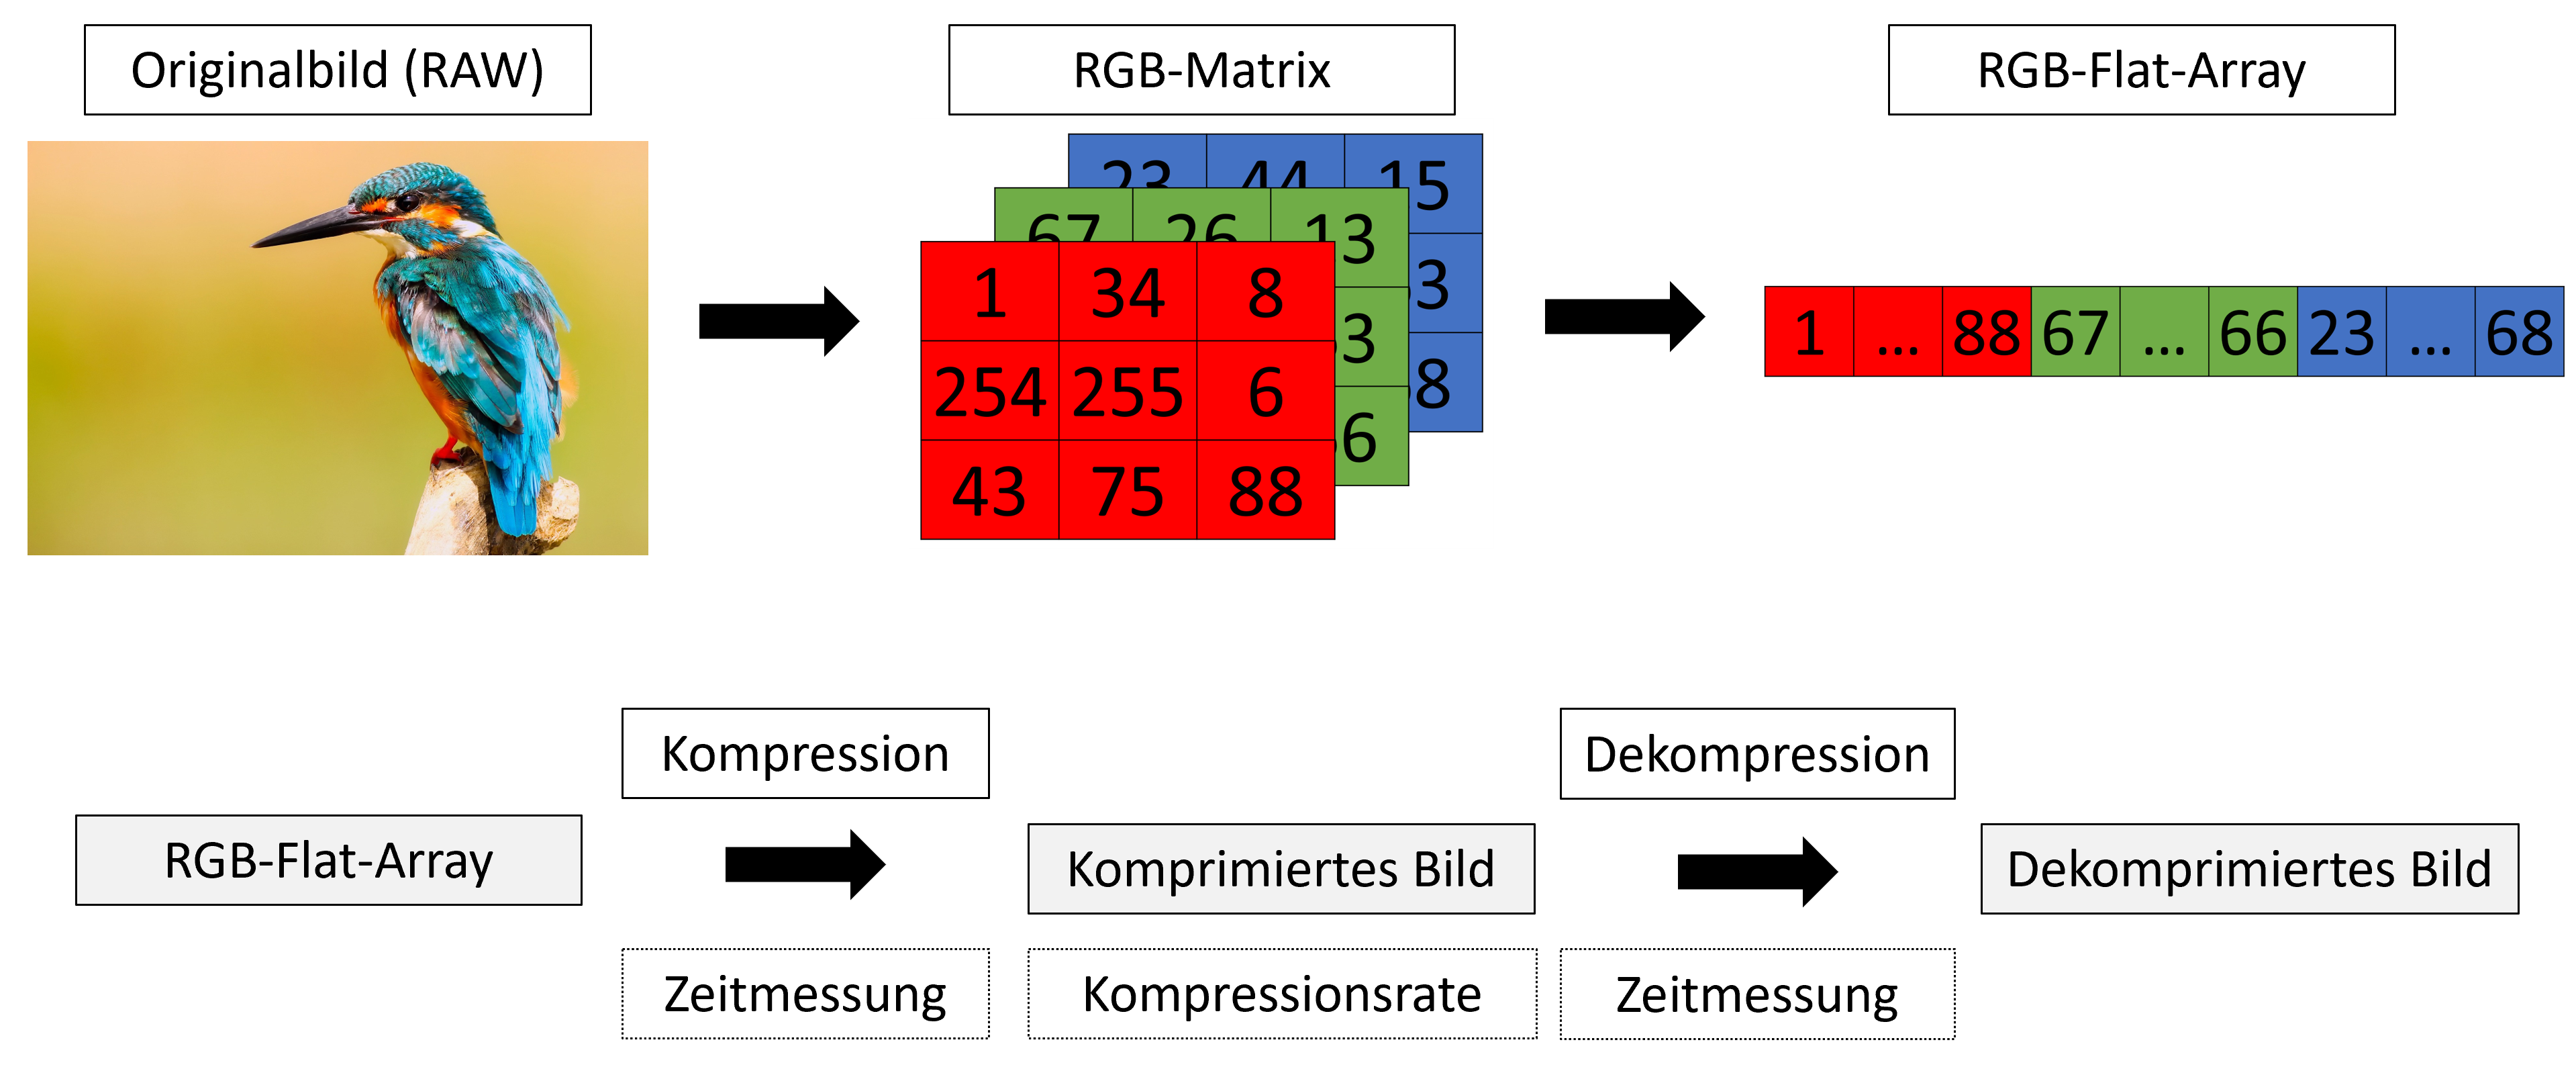
\includegraphics[width=\columnwidth]{./images/Idea.png}
    \caption{Umsetzung des Versuchs}
\end{figure}

Abbildung \ref{fig:idea} zeigt den Aufbau des Versuchs.
Die erste Zeile zeigt wie das Eingangsbild in das benötigte Format umgewandelt 
wird.
Das Origanlbild das komprimiert werden soll ist unkomprimiert und unbearbeitet.
Es wird im ersten Schritt in eine RGB Matrix umgewandelt.
Diese Umwandlung ist vom Originalbild zur Matrix, aber auch von der Matrix 
zum Originalbild möglich und ist eindeutig umkehrbar.
Die Matrix hat die Form (Pixelbreite Originalbild, Pixelhöhe Originalbild, 
3 Farbkanäle).
Jeder der drei Farbkanäle (rot, grün, blau) beschreibt eine zweidimensionale Matrix, 
die für jeden Pixel den Wert der entsprechenden Farbe angibt.
Im nächsten Schritt wird aus der Matrix eine Flache Liste gemacht.
Dazu werden alle Werte der Farbkanäle aneinandergereiht.
Zuerst alle Werte von Kanal rot, dann grün, dann blau.

% todoasdf
Algorithmen für Text ausgelegt, Liste mit Werte zwischen 0,255, 1-Dimensional
--> können von Algorithmen die Text komprimieren können komprimiert werden.



Die nächste Zeile in Abbildung \ref{fig:idea} beschreibt den Programmablauf.
Liste von Bild weiter gearbeitet.








Umsetzung in Python, high level programming language, schnell umsetzbar, aber nicht
Laufzeitoptimiert
Vereinfachungen/ Annahmen getroffen:
- keine Optimierungen der Algorithmen,
- 8-Bit Farbinformationen,




\section{Vorstellung der Algorithmen}


\section{Wahl der Testbilder}

\begin{figure}[h]
  \label{fig:testbilder}
  \centering
  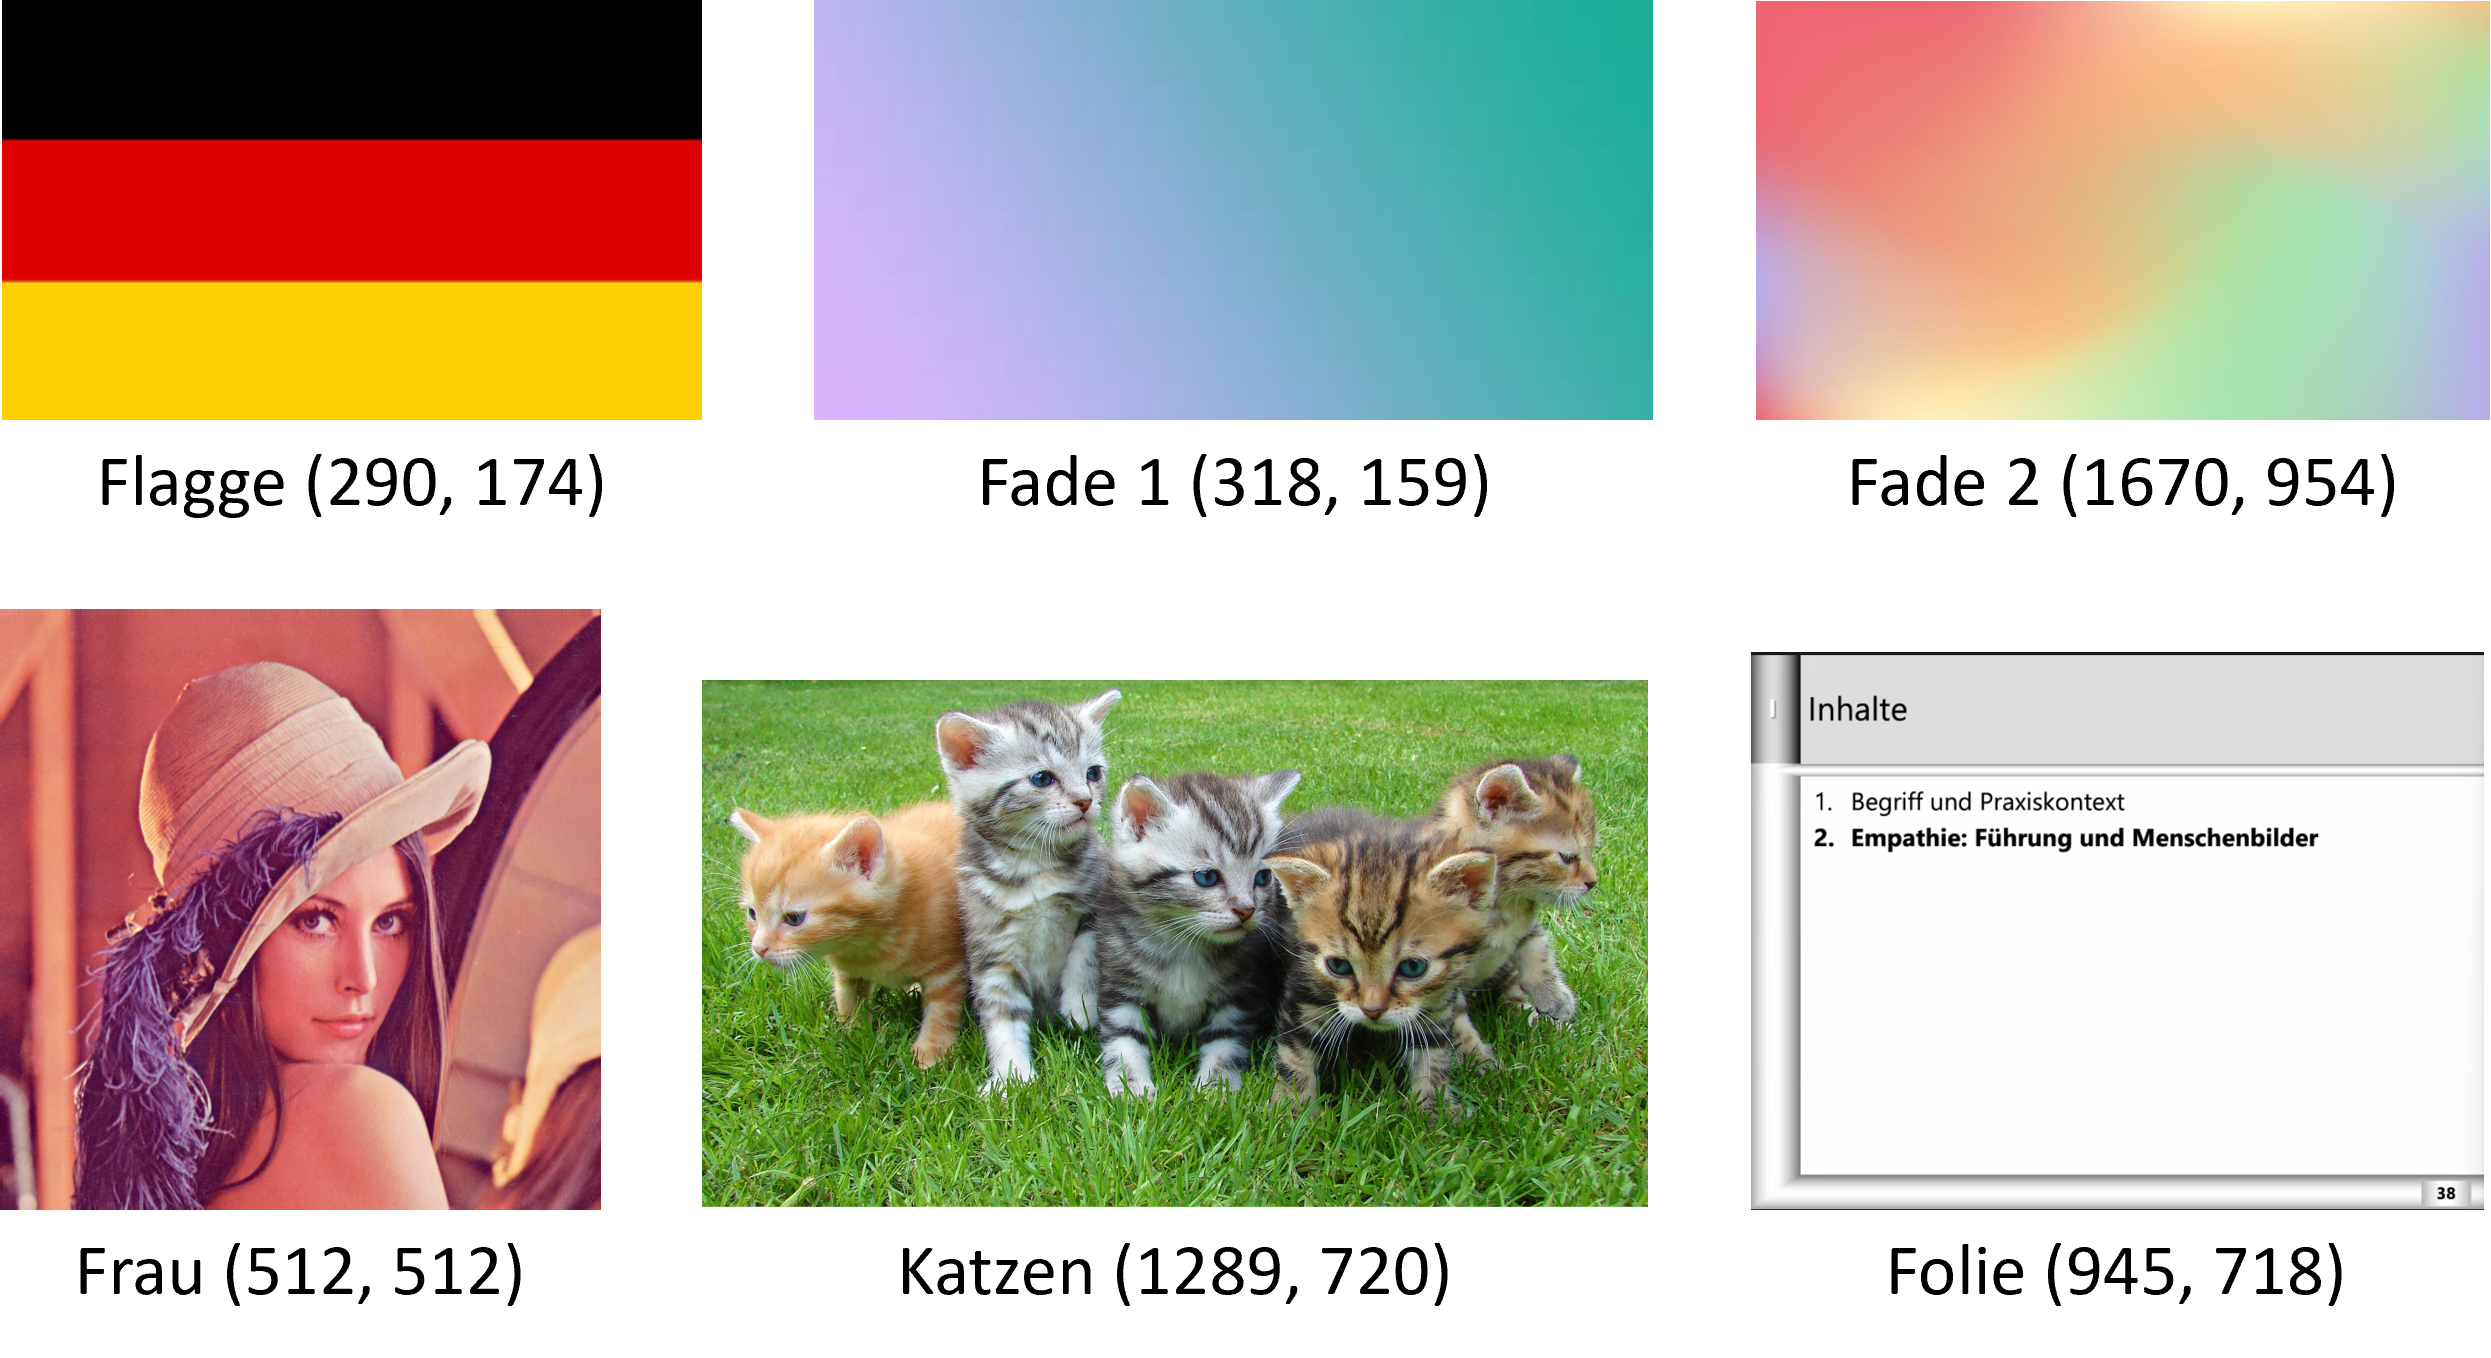
\includegraphics[width=\columnwidth]{./images/Images.png}
  \caption{Testbilder mit Auflösung}
\end{figure}



\section{Ergebnisse und Interpretation}

\begin{table*}
  \renewcommand*{\arraystretch}{1.1}
  \centering
  \begin{threeparttable}
    \caption{Kompressionsraten}
    \label{tab:komprate}
      \begin{tabular}{c *9{c} S[table-format=5.9]}

      \toprule
      Name    &  Auflösung  & RLE   & Huffman   & LZ77  & Deflate   & Filter + Huffman  & Filter + LZ77     & PNG   \\
      \midrule
      Flagge  & (290, 174)  & 99,98  & 77,85     & 78,85  & 91,70     & 87,38             & 84,69             & 91,80  \\
      Fade 1  & (318, 159)  & 45,73  & 14,30     & 25,87  & 31,90     & 84,94             & 78,13             & 80,69  \\
      Frau    & (512, 512)  & -39,19 & 2,74      & -10,96 & -9,51     & 38,22             & -7,41             & 3,38   \\
      Folie   & (945, 718)  & 84,57  & 56,87     & 73,48  & 76,62     & 84,90             & 81,66             & 87,03  \\
      Katzen  & (1289, 720) & -42,85 & 2,11      & -11,39 & -9,31     & 25,49             & -10,42            & -2,45  \\ 
      Fade 2  & (1670, 954) & 78,95  & 10,95     & 62,13  & 66,95     & 85,74             & 80,59             & 83,74          
    \end{tabular}
    \par\tnote{1} Angaben in Prozent, gerundet auf zwei Nachkommastellen
    \par\tnote{2} Bilder nach Größe aufsteigend sortiert
  \end{threeparttable}
\end{table*}


\begin{table*}
    \renewcommand*{\arraystretch}{1.1}
    \centering
    \begin{threeparttable}
      \caption{Kompressionszeiten}
      \label{tab:kompzeiten}
        \begin{tabular}{c *9{c} S[table-format=5.9]}

        \toprule
        Name    &  Auflösung  & RLE   & Huffman   & LZ77  & Deflate   & Filter + Huffman  & Filter + LZ77     & PNG   & Filter\\
        \midrule
        Flagge  & (290, 174)  & 0,015 & 0,017     & 2,3   & 2,3       & 1,3               & 3,3               & 3,3   & 1,3       \\
        Fade 1  & (318, 159)  & 0,028 & 0,018     & 14    & 14        & 1,6               & 5                 & 5     & 1,6       \\
        Frau    & (512, 512)  & 0,21  & 0,09      & 139   & 139       & 9                 & 131               & 131   & 9         \\
        Folie   & (945, 718)  & 0,47  & 0,24      & 63    & 63        & 22                & 62                & 62    & 22        \\
        Katzen  & (1289, 720) & 0,77  & 0,33      & 530   & 530       & 32                & 540               & 540   & 32        \\ 
        Fade 2  & (1670, 954) & 0,61  & 0,55      & 200   & 200       & 51                & 140               & 140   & 51        
      \end{tabular}
      \par\tnote{1} Angaben in Sekunden
      \par\tnote{2} Bilder nach Größe aufsteigend sortiert
      \par\tnote{3} Die Spalte Filter gibt die Filterzeit an
    \end{threeparttable}
  \end{table*}


  \begin{table*}
    \renewcommand*{\arraystretch}{1.1}
    \centering
    \begin{threeparttable}
      \caption{Dekompressionszeiten}
      \label{tab:dekompzeiten}
        \begin{tabular}{c *9{c} S[table-format=5.9]}

        \toprule
        Name    &  Auflösung  & RLE     & Huffman   & LZ77  & Deflate   & Filter + Huffman  & Filter + LZ77     & PNG       & Revert Filter \\
        \midrule
        Flagge  & (290, 174)  & 0,003   & 0,012     & 0,120 & 0,124     & 0,124             & 0,255             & 0,255     & 0,120       \\
        Fade 1  & (318, 159)  & 0,032   & 0,048     & 3,5   & 3,5       & 0,008             & 0,500             & 0,550     & 0,220       \\
        Frau    & (512, 512)  & 0,395   & 0,293     & 308   & 308       & 1,4               & 230               & 230       & 1,4         \\
        Folie   & (945, 718)  & 0,769   & 0,321     & 82    & 82        & 3                 & 35                & 35        & 2,9        \\
        Katzen  & (1289, 720) & 1,4     & 1         & 1200  & 1200      & 5,1               & 1205              & 1205      & 5          \\ 
        Fade 2  & (1670, 954) & 0,480   & 1,5       & 732   & 732       & 7                 & 184               & 184       & 7        
      \end{tabular}
      \par\tnote{1} Angaben in Sekunden
      \par\tnote{2} Bilder nach Größe aufsteigend sortiert
      \par\tnote{3} Die Spalte Revert Filter gibt die Zeit an, in der die Filterung rückgängig gemacht wird
    \end{threeparttable}
  \end{table*}





\section{Finale Auswertung}


\bibliographystyle{IEEEtran}
\bibliography{mybib}

\end{document}
